\documentclass{article}
\usepackage[paperwidth=210mm,paperheight=297mm, top = 30mm, bottom = 30mm]{geometry}
%\usepackage[hangul]{kotex}
\usepackage{kotex}
\usepackage[utf8]{inputenc}
\usepackage{enumitem}
\usepackage{indentfirst}
\usepackage{graphicx, subcaption, tikz}
\usepackage{amsmath, amssymb, amsthm, amsfonts, bm}
\usepackage{listings}

\title{2020 Spring MAS365 Numerical Analysis HW6}
\author{20160650 채지석}
\date{\today}

\setlist{  
  listparindent=\parindent,
  %parsep=0pt,
}

\lstset{frame=tb,
  language=Python,
  aboveskip=3mm plus 2mm,
  belowskip=3mm plus 2mm minus 2mm,
  showstringspaces=false,
  columns=flexible,
  basicstyle={\small\ttfamily},
  numbers=none,
  %numberstyle=\tiny\color{gray},
  %keywordstyle=\color{blue},
  %commentstyle=\color{dkgreen},
  %stringstyle=\color{mauve},
  breaklines=true,
  breakatwhitespace=true,
  frame=single,
  tabsize=4
}

\newtheorem{prob}{Problem}

\newcommand{\set}[1]{\left\{ {#1} \right\}}
\newcommand{\vecx}{\boldsymbol{x}}
\newcommand{\mat}[1]{\boldsymbol{#1}}
\newcommand{\mata}{\boldsymbol{A}}
\newcommand{\matb}{\boldsymbol{B}}
\newcommand{\rr}{\mathbb{R}}
\newcommand{\nn}{\mathbb{N}}
\newcommand{\zz}{\mathbb{Z}}
\newcommand{\cc}{\mathbb{C}}
\newcommand{\qq}{\mathbb{Q}}
\newcommand{\norm}[1]{\left\lVert#1\right\rVert}
\newcommand{\card}[1]{\left\lvert#1\right\rvert}
\newcommand{\posdef}{\succ\mat{0}}
\newcommand{\psd}{\succeq\mat{0}}
\newcommand{\trace}{\text{trace}}
\newcommand{\comment}[1]{}
\newcommand{\problem}{\begin{prob}\end{prob}}
                    

\begin{document}

\section*{Computer Assignment}
The program which does the required is submitted via KLMS along with this document. As it is a continuation of assignment 7, the first ~130 lines of the code is almost identical with assignment 7.

The QR method is implemented, following the rules (6.6.4.3) of the textbook. Performing the QR decomposition is done using the \texttt{numpy} built-in function \texttt{numpy.linalg.qr}, although we also provide a self-made function \texttt{my\_qr} which is capable of performing QR decomposition. However as expected, \texttt{my\_qr} is much slower than \texttt{numpy.linalg.qr}, so practically we should use that instead of \texttt{my\_qr}.

The stopping criteria is, as always, based on the relative error. This time we deal with matrices, so matrix norms are used in place of vector norms. Threshold is set to be $10^{-6}$, also as always.

As mentioned in Theorem 6.6.4.15 of the textbook, QR iteration may not converge in general. Luckily in our case we see a convergence, but when we have no convergence the stopping criteria using relative error may not work properly. So this time, we also set a limit on the maximum number of iterations. Default value of this limit is set to be 1000.

To see if the QR iteration has converged or not we print out the maximum aboslute value of the off-diagonal entries. If the QR iteration has converged then the result will be close to a diagonal matrix, so this output indicates the convergence. Also it is required to compare the resulting eigenvalues with the results from assignment 7, so we compute the relative errors for each computed eigenvalues.

\begin{center}
    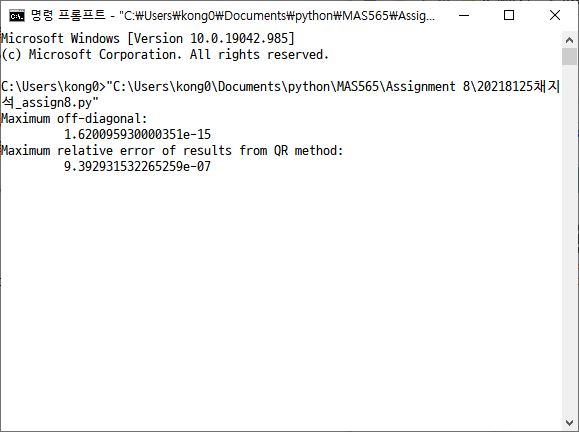
\includegraphics[width=0.75\linewidth]{console.JPG}
\end{center} 

The results imply that the QR method has converged well, and the computed eigenvalues are not much different from the eigenvalues computed in assignment 7, which is where we computed the eigenvalues using the built-in method \texttt{numpy.linalg.eig}. 

To have a better visual explanation on how well our QR method has performed we plot the two results, as the following figure. With our naked eye the two plots are nearly indistinguishable.

\begin{figure*}[th]
  \centering
  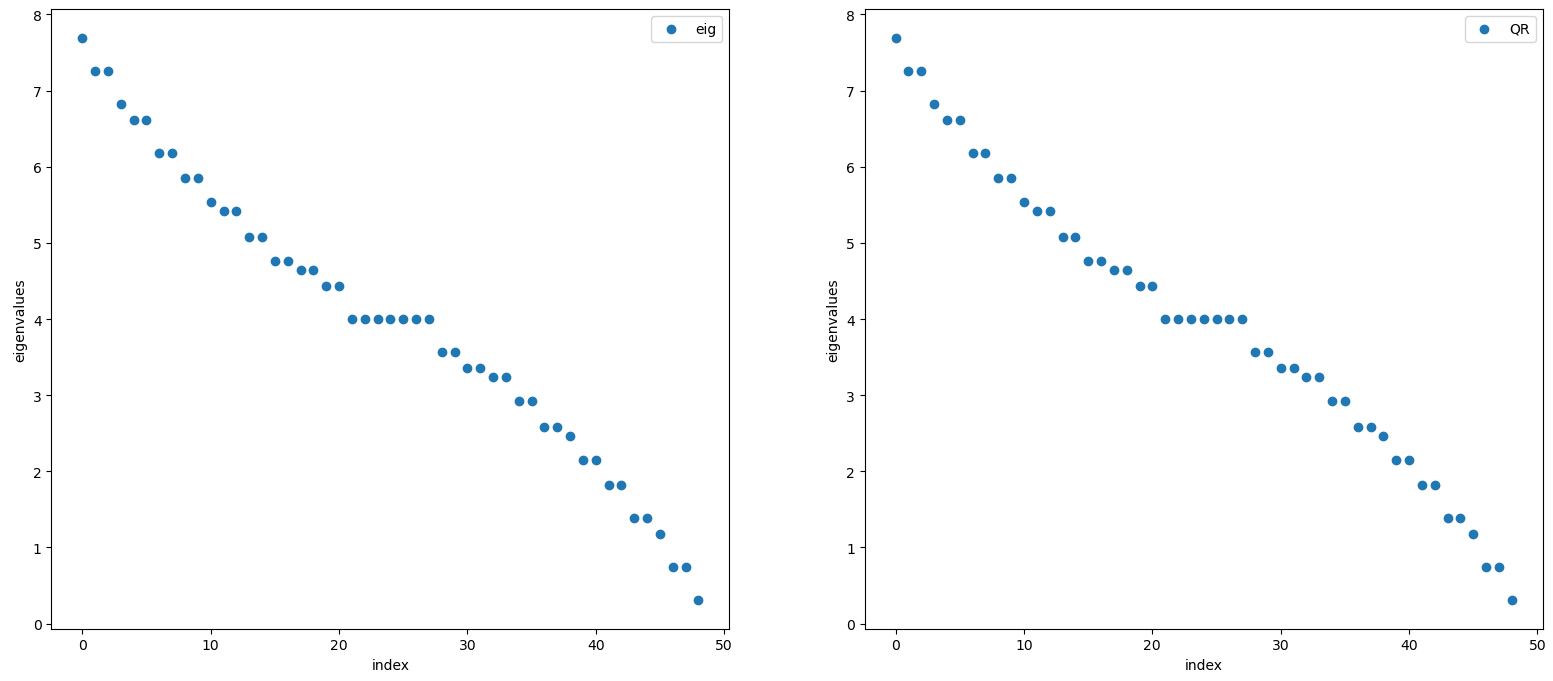
\includegraphics[width=0.95\textwidth]{3313.png}
  \caption{Scatter plots of the eigenvalues computed by \texttt{eig}(left) and the QR method(right)}
  \label{fig:mean and std of net14}
\end{figure*}
  
\end{document}